\documentclass[12pt]{article}
 
\usepackage[margin=1in]{geometry} 
\usepackage{amsmath,amsthm,amssymb}
\usepackage{enumitem} 
\usepackage{graphicx}
\graphicspath{ {./images/} }


\newcommand{\problem}[1]{
	\vskip 1em
	{\large \textbf{#1}}
}
 
\begin{document}

\title{CS 1511 Homework 10} % Replace X with the appropriate number
\author{Mathew Varughese, Justin Kramer, Zach Smith} 
\date{Wednesday, Feb 20}

\maketitle


\setlength{\parskip}{.2em}
\setlength\parindent{0pt}
 
\problem{18. a}
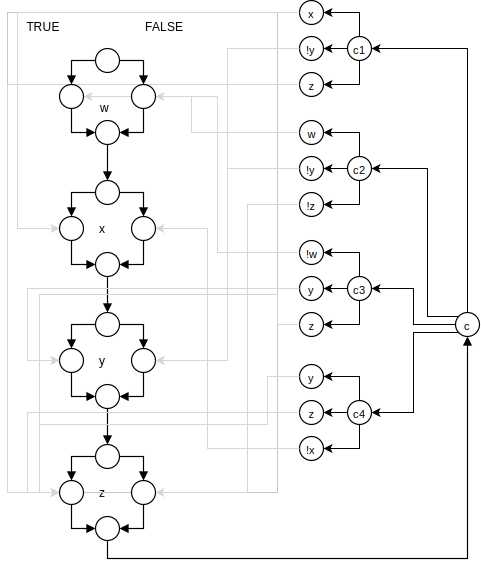
\includegraphics[width=5.5in]{18a}
 
\problem{18. b}


Based on this reduction and diagram, player 2 would have 
the winning strategy
if you could pick variables to satisfy the QBF. 

In the table, we see that each row needs to evaluate to true
for the full expression to true. 

Say w = T, then y must be T to make the third row work. Then, the
first row will not be satisfied because x and z could be anything, 
which would make it false. 

Say w = F. Then y must be True. The same problem applies, the first 
row will be false since x and z could be anything. 

w can either be T or F, and since both options lead to 
the expression being false, there 
is not a way to make this formula true. Therefore, 
this problem is not in TBQF, so by the reduction we created 
Player 2 would have the winning strategy.

\begin{table}[]
\begin{tabular}{llll}
$\exists$  & $\forall$  & $\exists$  & $\forall$  \\
	& x  & !y & z  \\
w  &    & !y & !z \\
!w &    & y  & z  \\
	& !x & y  & z 
\end{tabular}
\end{table}



\end{document}